\chapter{Πειραματική Εφαρμογή}
\label{chap5}

\section{Δεδομένα}

Στη διάθεση μας έχουμε ένα σύνολο δεδομένων που περιγράφουν την στάθμη υγρού φυσικού αερίου σε ένα σύνολο δεξαμενών στη Γαλλία. Ο αρχικός σκοπός της ανάλυσης ήταν να μπορέσουμε να προβλέψουμε πότε αυτές οι δεξαμενές θα αδειάσουν λόγω της κατανάλωσης έτσι ώστε η εταιρεία να φροντίσει να ανεφοδιαστούν. Με αυτό τον τρόπο θα αποφευχθεί οποιαδήποτε πρόβλημα με τους καταναλωτές αλλά συγχρόνως θα επιτραπεί στην εταιρεία να σχεδιάσει κατά βέλτιστο τρόπο την διαδικασία αναπλήρωσης υγρού φυσικού αερίου στις δεξαμενές.

Τα δεδομένα ξεκινούν τον Αύγουστο του 2012 και συνεχίζουν ως και τον Νοέμβρη του 2015. H συχνότητα μεταξύ των παρατηρήσεων κυμαίνεται από μερικές ώρες σε αρκετές μέρες μέχρι την επόμενη παρατήρηση. Περιγράφουν όγκο, άρα και η μονάδα που τα περιγράφει είναι αντίστοιχα μονάδα μέτρησης όγκου. 

\section{Προετοιμασία Χρονοσειρών}

Παρατηρούμε ότι τα δεδομένα δεν χαρακτηρίζονται από σταθερή συχνότητα δειγματοληψίας, ούτε μεταξύ του αλλά ούτε κατά μήκος της χρονοσειράς που περιγράφει καθένα από αυτά. Χαρακτηριστικό παράδειγμα είναι χρονοσειρές που μπορεί για κάποιες ημέρες να έχουν πολλές παρατηρήσεις, ενώ σε άλλες να ακολουθεί μεγάλο διάστημα μέχρι την επόμενη μέρα που έχουμε δεδομένα.

Τα δεδομένα προέκυψαν από αισθητήρες εντός των δεξαμενών, που παρήγαγαν δεδομένα σε διαφορετικές στιγμές για κάθε δεξαμενή. Επίσης, υπήρχε περίπτωση σφάλματος στη μέτρηση, με τη στάθμη να μετράται μεγαλύτερη από κάποια προηγούμενη χρονική στιγμή, χωρίς να έχει συμβεί ανεφοδιασμός ανάμεσα.

Επίσης στα δεδομένα είναι εμφανείς οι χρονικές στιγμές που έγινε ανεφοδιασμός, καθώς βλέπουμε μια αλλαγή επιπέδου στη χρονοσειρά που τα περιγράφει, όπως φαίνεται στο Σχήμα \ref{originalTS}. Στη συγκεκριμένη χρονοσειρά, παρατηρούμε ότι μεγάλο πλήθος από ανεφοδιασμούς στο χρονικό διάστημα για το οποίο έχουμε πληροφορία. 

\begin{figure}[t!]
  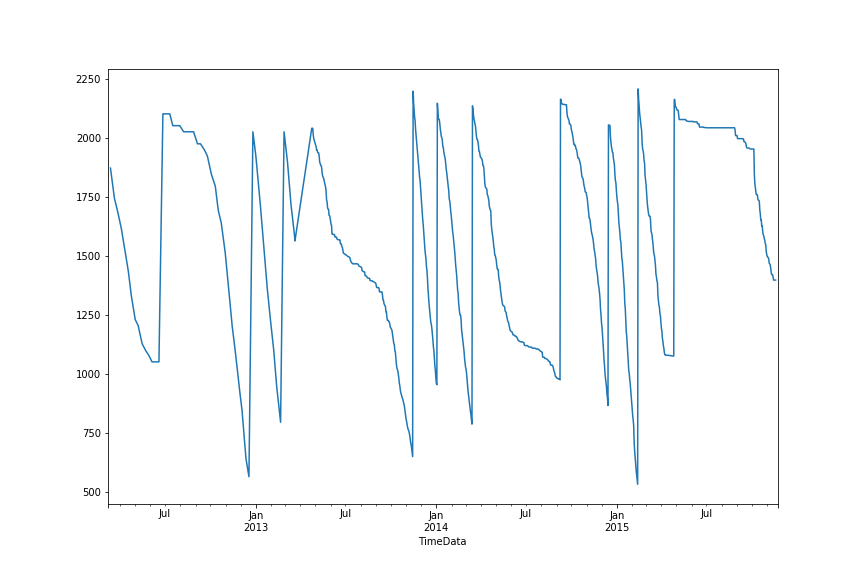
\includegraphics[scale=0.5]{figures/original.png}
\centering
\caption{Χρονοσειρά επιπέδου υγρού φυσικού αερίου σε δεξαμενή}
\label{originalTS}
\end{figure} 

Λόγω της φύσης της πληροφορίας που έχουμε, γνωρίζουμε ότι καμία στιγμή, σε ενεργές δεξαμενές δε μπορούμε να έχουμε μηδενικές τιμές και προφανώς δεν μπορεί μία δεξαμενή να έχει αρνητικό όγκο φυσικού αερίου. 

Τα παραπάνω μας οδηγούν στο να κάνουμε τις εξής ενέργειες για τη προετοιμασία των χρονοσειρών:

\begin{itemize}
    \item Μετατρέπουμε τυχούσες μη θετικές τιμές σε κενές τιμές
    \item Φέρνουμε τα δεδομένα σε επίπεδο ημέρας κρατώντας, στις περιπτώσεις πολλαπλών παρατηρήσεων, τη μικρότερη από αυτές
    \item Συμπληρώνουμε τις κενές τιμές με τη μέθοδο της γραμμικής παρεμβολής βάσει του χρόνου 
     \end {itemize}
     
Στόχος μας, όμως, εν τέλει είναι να προβλέψουμε πότε η δεξαμενή θα αδειάσει. Για να το εντοπίσουμε αυτό πρέπει να εστιάσουμε τη προσοχή μας στο ρυθμό κατανάλωσης της χρονοσειράς. Έτσι, χρησιμοποιούμε πρώτες διαφορές στα δεδομένα για να δούμε τι κατανάλωση είχαμε μέσα σε μία μέρα. Σε αυτό το σημείο, παρατηρούμε ότι τις ημέρες που είχαμε refills η χρονοσειρά μας παρουσιάζει ακραίες τιμές που δεν ανταποκρίνονται στον φυσιολογικό ρυθμό κατανάλωσης που χαρακτηρίζει τη δεξαμενή. Συνεπώς, θέτουμε εκείνη την ημέρα σας κενή τιμή και ξαναχρησιμοποιούμε τη μέθοδο της παρεμβολής για να τη διαχειριστούμε.

Επίσης, σκοπός μας είναι να γνωρίζουμε αρκετά πριν πότε μέλλεται μία δεξαμενή να αδειάσει. Βγάζει λοιπόν περισσότερο νόημα να χρησιμοποιήσουμε τα μοντέλα μας για να προβλέψουμε τη μηνιαία κατανάλωση. Έτσι, φέρνουμε τα δεδομένα σε επίπεδο μήνα, παίρνοντας τον μέσο όρο της ημερήσιας κατανάλωσης και λαμβάνουμε τη χρονοσειρά της μηνιαίας κατανάλωσης.

Στο Σχήμα \ref{originalmonthlyTS} βλέπουμε τη νέα μορφή των δεδομένων για την ίδια δεξαμενή. Η ετήσια εποχιακή συμπεριφορά της χρονοσειράς είναι πλέον εμφανής.

\begin{figure}[t!]
  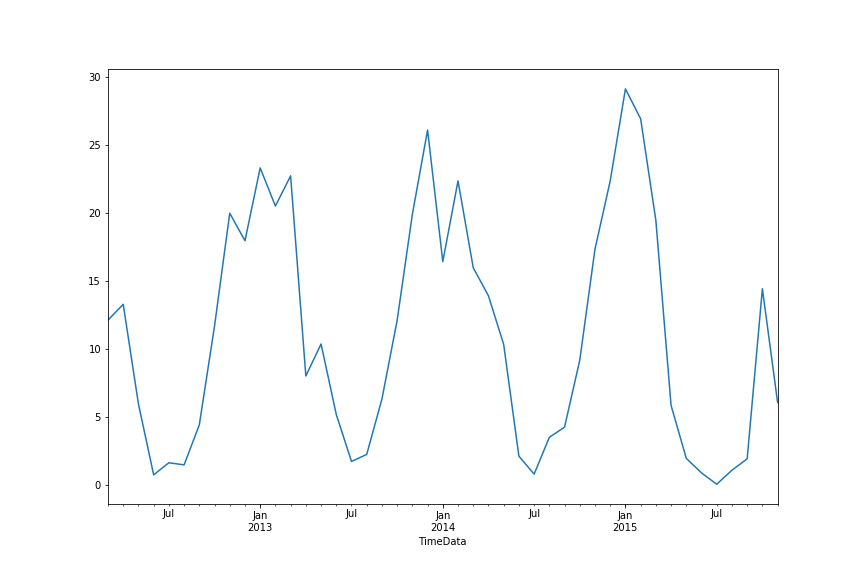
\includegraphics[scale=0.5]{figures/originalmonthly.png}
\centering
\caption{Χρονοσειρά μέσης μηνιαίας κατανάλωσης}
\label{originalmonthlyTS}
\end{figure} 

Τελικώς, για να μπορούμε αξιολογήσουμε τη μέθοδο πρόβλεψης, αποκρύβουμε τις 6 τελευταίες παρατηρήσεις για να τις χρησιμοποιήσουμε ως ορίζοντα πρόβλεψης

\section{Αποεποχικοποίηση}

Όπως περιγράψαμε στο κεφάλαιο της μεθοδολογίας, χωρίζουμε τις χρονοσειρές σε δύο κατηγορίες: αυτές που έχουν πάνω από τρία έτη παρατηρήσεις και αυτές που έχουν λιγότερες.  

Ακολουθώντας έτσι την μεθοδολογία της κλασσικής μεθόδου αποσύνθεσης με το πολλαπλασιαστικό μοντέλο και της συρρίκνωσης συντελεστών με τη μέθοδο \en{James-Stein} λαμβάνουμε τους εποχιακούς δείκτες για τις χρονοσειρές τις πρώτης ομάδας. Μπορούμε να δούμε την εποχιακότητα της χρονοσειράς των προηγούμενων σχημάτων στο Σχήμα \ref{seasonality}.

\begin{figure}[t!]
  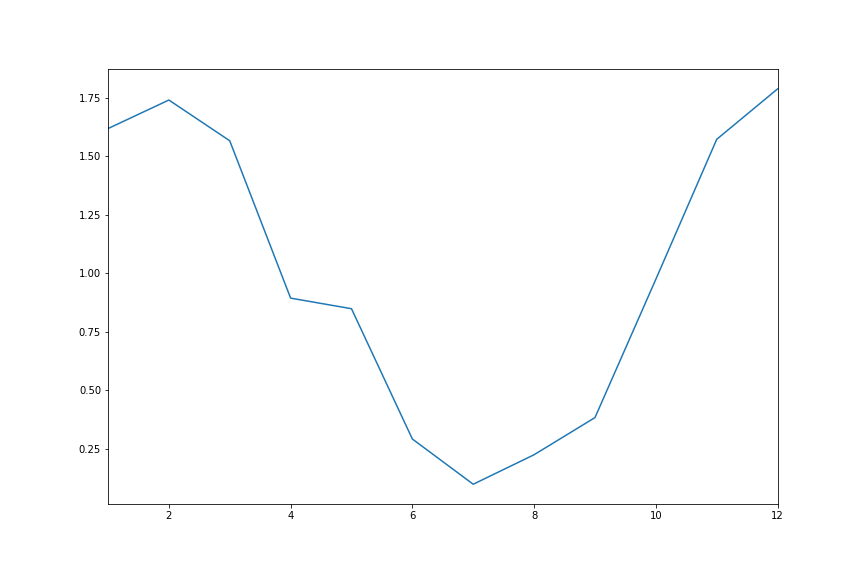
\includegraphics[scale=0.5]{figures/seasonality.png}
\centering
\caption{Δείκτες εποχιακότητας}
\label{seasonality}
\end{figure} 

Αντίστοιχα στο Σχήμα \ref{pseudoseasonality} βλέπουμε το αποτέλεσμα του υπολογισμού της ψευδο-εποχιακότητας σε μία χρονοσειρά.


\begin{figure}[t!]
  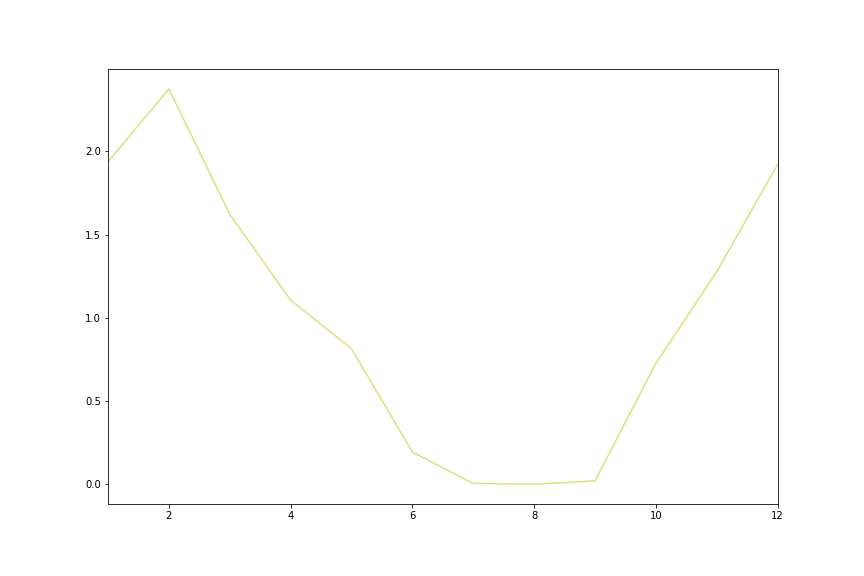
\includegraphics[scale=0.5]{figures/pseudoseasonality.png}
\centering
\caption{Δείκτες ψευδο-εποχιακότητας}
\label{pseudoseasonality}
\end{figure} 

Παρατηρούμε ότι τα αποτελέσματα των δύο κινούνται στην ίδια κλίμακα, και συνεπώς μπορούν να είναι συγκρίσιμα και να μας επιτρέψουν να φτιάξουμε τις συστάδες κατά τον τρόπο που περιγράψαμε στο προηγούμενο κεφάλαιο. 

\section{Συσταδοποίηση Δεικτών Εποχιακότητας}

Χρησιμοποιώντας τον αλγόριθμο \en{DBSCAN} στους δείκτες εποχιακότητας των χρονοσειρών με επαρκείς παρατηρήσεις προέκυψε η διαμέριση που φαίνεται στο Σχήμα \ref{DBSCANresults}, με το τελευταίο σύνολο να μην μπορεί να δημιουργήσει συστάδες.

\begin{figure}[t!]
  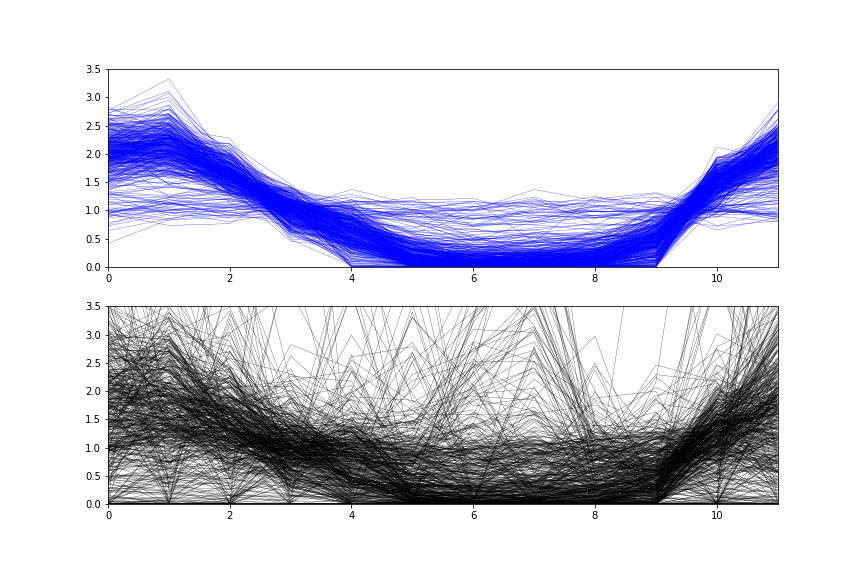
\includegraphics[scale=0.5]{figures/dbscan.png}
\centering
\caption{Συσταδοποίηση δεικτών εποχιακότητας}
\label{DBSCANresults}
\end{figure} 

Βλέπουμε ότι ένα μεγάλο πλήθος χρονοσειρών δεν παρουσιάζει συνάφεια με άλλες χρονοσειρές. Δοκιμάζοντας διαφορετικές τιμές στις παραμέτρους του αλγορίθμου, προκύπτουν περισσότερες συστάδες με μεγαλύτερη πυκνότητα αλλά με μικρότερο πλήθος χρονοσειρών η κάθε μία. Αφότου, όμως σκοπεύουμε να χρησιμοποιήσουμε το αποτέλεσμα για μάθουμε την εποχιακή συμπεριφορά του συνόλου των δεδομένων μας πρέπει να αποφύγουμε την υπερ-προσαρμογή (\en{overfitting}) σε συγκεκριμένα μοτίβα.

Το επόμενο βήμα είναι να υπολογίσουμε το κέντρο της συστάδας, το οποίο λάβαμε υπολογίζοντας τη μέση τιμή των δεικτών εποχιακότητας που ανήκουν σε αυτή. Το αποτέλεσμα φαίνεται στο Σχήμα \ref{centroid}.

\begin{figure}[t!]
  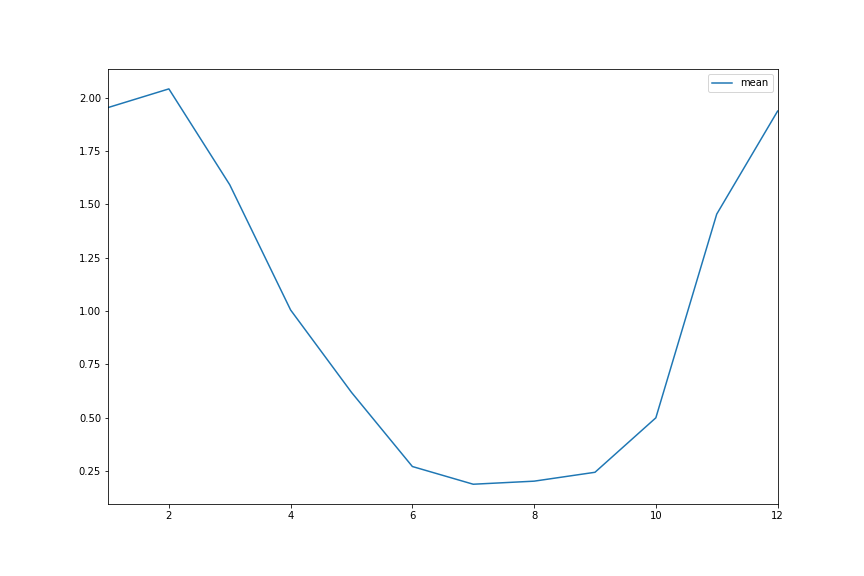
\includegraphics[scale=0.5]{figures/centroid.png}
\centering
\caption{Δείκτες εποχιακότητας κέντρου συστάδας}
\label{centroid}
\end{figure} 

Υπολογίζουμε, κατόπιν τη μέγιστη τετραγωνική διαφορά μεταξύ των δεικτών εποχιακότητας του \en{cluster} και του κέντρου του. Ελέγχουμε κάθε σύνολο δεικτών ψευδο-εποχιακότητας αν έχει απόσταση μικρότερη της μέγιστης διαφοράς που υπολογίσαμε. Οι χρονοσειρές που πληρούν αυτό το κριτήριο φαίνονται στο Σχήμα \ref{pseudocentroid} μαζί με το κέντρο της συστάδας.

\begin{figure}[t!]
  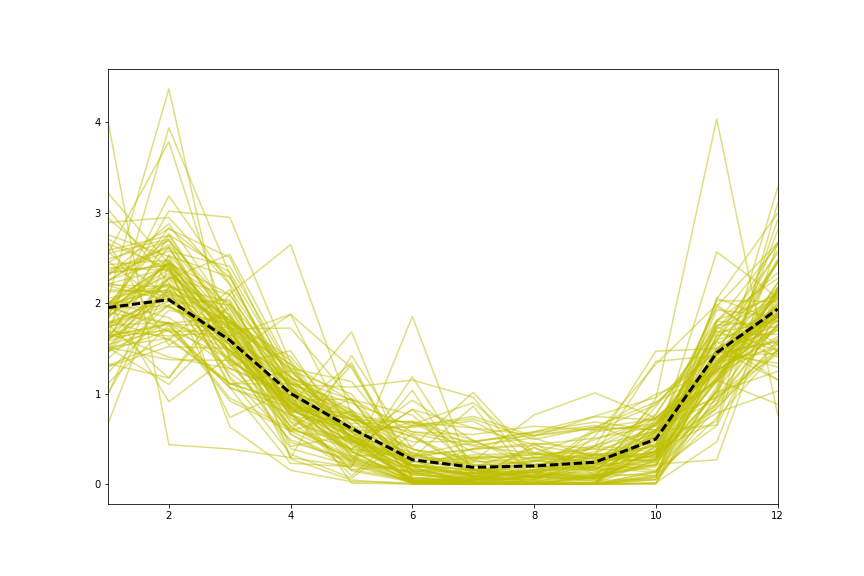
\includegraphics[scale=0.5]{figures/pseudocentroid.png}
\centering
\caption{Δείκτες ψευδο-εποχιακότητας συστάδας}
\label{pseudocentroid}
\end{figure} 

\section{Πρόβλεψη}

Έχοντας εντοπίσει τις χρονοσειρές που μας ενδιαφέρουν, τις προεκτείνουμε στο μέλλον με δύο τρόπους:

\begin{enumerate}
    \item Πρόβλεψη της αρχικής χρονοσειράς
    \item \begin{enumerate}
	\item Αποεποχικοποίηση με τους κεντρικούς δείκτες
	\item Πρόβλεψη
	\item Επαναεποχικοποίηση
      \end{enumerate}
      \end{enumerate}
 
Βλέπουμε τα αποτελέσματα της πρώτης μεθόδου στο Σχήμα \ref{classicforecasting} για μία από τις χρονοσειρές. Για την ίδια, τα αποτελέσματα της προτεινόμενης μεθόδου φαίνονται στα Σχήματα \ref{deseasonalizedforecast} και \ref{newforecasting}, για την αποεποχικοποιημένη και τελική πρόβλεψη αντίστοιχα.


\begin{figure}[t!]
  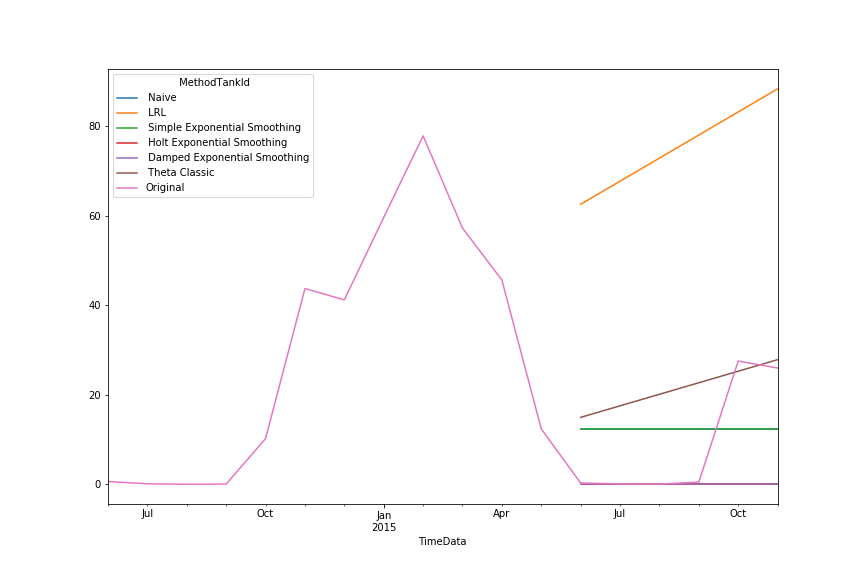
\includegraphics[scale=0.5]{figures/classicforecasting.png}
\centering
\caption{Πρόβλεψη κλασικής προσέγγισης}
\label{classicforecasting}
\end{figure} 


\begin{figure}[t!]
  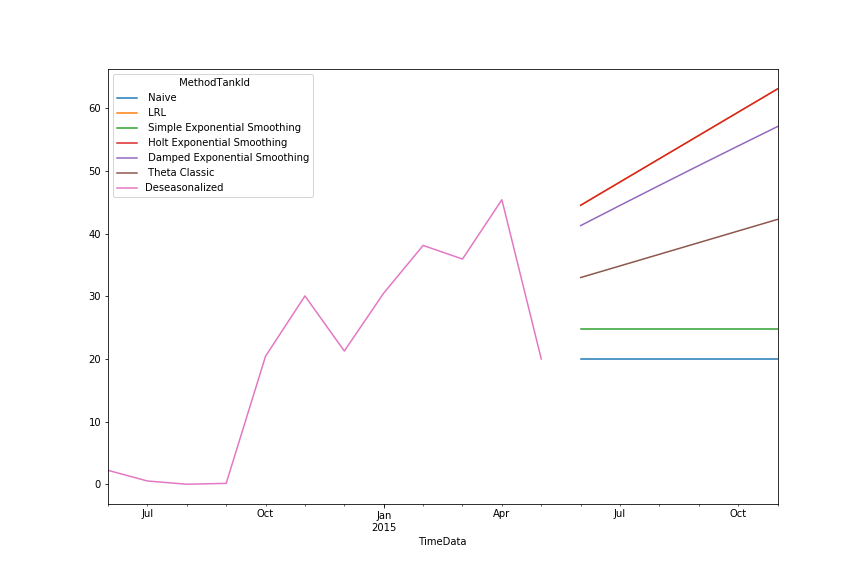
\includegraphics[scale=0.5]{figures/deseasonalized.png}
\centering
\caption{Πρόβλεψη αποεποχικοποιημένης χρονοσειράς}
\label{deseasonalizedforecast}
\end{figure} 


\begin{figure}[t!]
  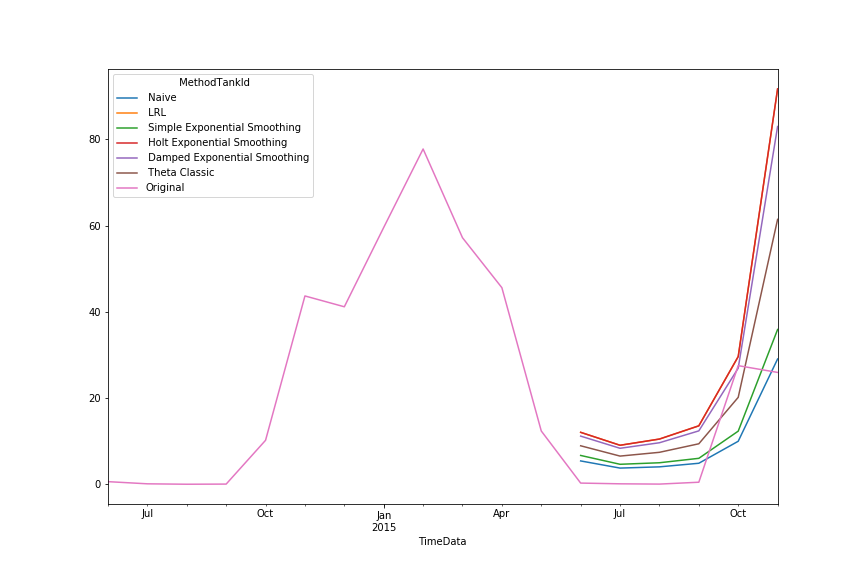
\includegraphics[scale=0.5]{figures/newforecasting.png}
\centering
\caption{Τελική πρόβλεψη προτεινόμενης προσέγγισης}
\label{newforecasting}
\end{figure} 

Πρέπει να σημειώσουμε ότι αφότου λάβαμε τα αποτελέσματα των προβλέψεων, οι τυχούσες αρνητικές τιμές μετατράπηκαν σε μηδενικές. Αυτό έγινε καθώς δε δύναται να έχουμε αρνητική κατανάλωση χωρίς εξωγενείς παράγοντες (π.χ. αναπλήρωση φυσικού αερίου), που μάλιστα τους έχουμε αφαιρέσει από την ανάλυση μας.

\section{Αξιολόγηση Μεθόδου}

Όπως περιγράψαμε στο τελευταίο βήμα του τελευταίου κεφαλαίου, μετράμε την ακρίβεια της μεθόδου με το κανονικοποιημένο μέσο απόλυτο σφάλμα. Μπορούμε να δούμε τα αποτελέσματα εν συνόλω για τη κάθε μέθοδο στον Πίνακα \ref{tab:results}. Η πρώτη στήλη δείχνει τις μεθόδους πρόβλεψης, η δεύτερη τον δείκτη ακρίβειας για τη κλασική προσέγγιση πρόβλεψης χρονοσειρών με μικρό ιστορικό, η τρίτη τον δείκτη ακριβείας για τη προτεινόμενη προσέγγιση και τελικώς φαίνεται το ποσοστό των υπό εξέταση χρονοσειρών που είχαμε καλύτερα αποτελέσματα με τη νέα μέθοδο.

\begin{table}[h]
  {
\centering
\begin{tabular}{|c|c|c|c|}
  \hline
  \textbf{Μέθοδος Πρόβλεψης} & \textbf{Κλασική} & \textbf{Προτεινόμενη} & \textbf{Ποσοστό (\%)} \\
  \hline
  \en{Naive}                    &    1.01     &  \textbf{0.81} &  70.97 \\
  \en{LRL}                    &        3.15 &  \textbf{0.99} &  94.74 \\
      \en{Simple Exponential Smoothing}   &  1.31 &  \textbf{1.02} &  74.74 \\ 
    \en{Holt Exponential Smoothing}   &   1.18 & \textbf{0.89} &  72.63 \\ 
    \en{Damped Exponential Smoothing}  &  1.05 & \textbf{0.93}  &  73.03 \\
    \en{Theta Classic}            &        1.22 &  \textbf{0.96} &  73.68 \\
    
  \hline
\end{tabular}
}
\caption{Ακρίβεια Μεθόδων}
\label{tab:results}
\end{table}

Τα αποτελέσματα μας δείχνουν ότι για το κατά πολύ μεγαλύτερο μέρος των χρονοσειρών τις προεκτείναμε με μεγαλύτερη ακρίβεια χρησιμοποιώντας ανάλυση συστάδων για αποεποχικοποίηση. Όλες οι μέθοδοι πρόβλεψης είχαν καλύτερα αποτελέσματα σε σύγκριση με τη κλασική προσέγγιση. 
